Before processing the datasets, ``gyrodometry" method is introduced in \cite{borenstein1996gyrodometry} referenced to determine the fused yaw angle change \(\Delta \psi\). One simple experiment is implemented to test on this method. The  bot  was  moved  along  a  groundtruth trajectory (Fig. \ref{fig:odometry_traj}), and the raw sensing data \(n_R\), \(n_L\), and \(\dot{\psi}_{IMU}\) were logged. \(R_R\), \(R_L\), and \(b\) were provided in the parameter sheet.

Based on the data measured on the robot, the yaw angle and angular velocity from pure wheel odometry and IMU, as well as their difference are shown in Fig. \ref{fig:odometry_angle_diff}. According to the figure, the typical range of the \(\dot{\psi}\) difference is within \(\pm\)0.5 rad/s. And the difference between \(\psi\) is generated mainly during the turning process, where the typical \(\dot{\psi}\) difference is within \(\pm\)0.3 rad/s. These show that a meaningful \(C_{\dot{\psi}}\) will be between 0-0.5 rad/s.

The gyrodometry was run on different \(C_{\dot{\psi}}\). According to the result in Fig. \ref{fig:odometry_tune}, always using yaw information from IMU leads to drift in the straight line period, while always using yaw information from wheel odometry leads to larger errors during turning. Choosing \(C_{\dot{\psi}} = 0.2\) rad/s will combine the strength of both the wheel odometry and IMU, and lead to result closer to the ground truth. Therefore, the \(C_{\dot{\psi}}\) is fixed, and the onboard result with this threshold is shown in Fig. \ref{fig:odometry_traj}.

\begin{figure}[hbt!]
    \centering
    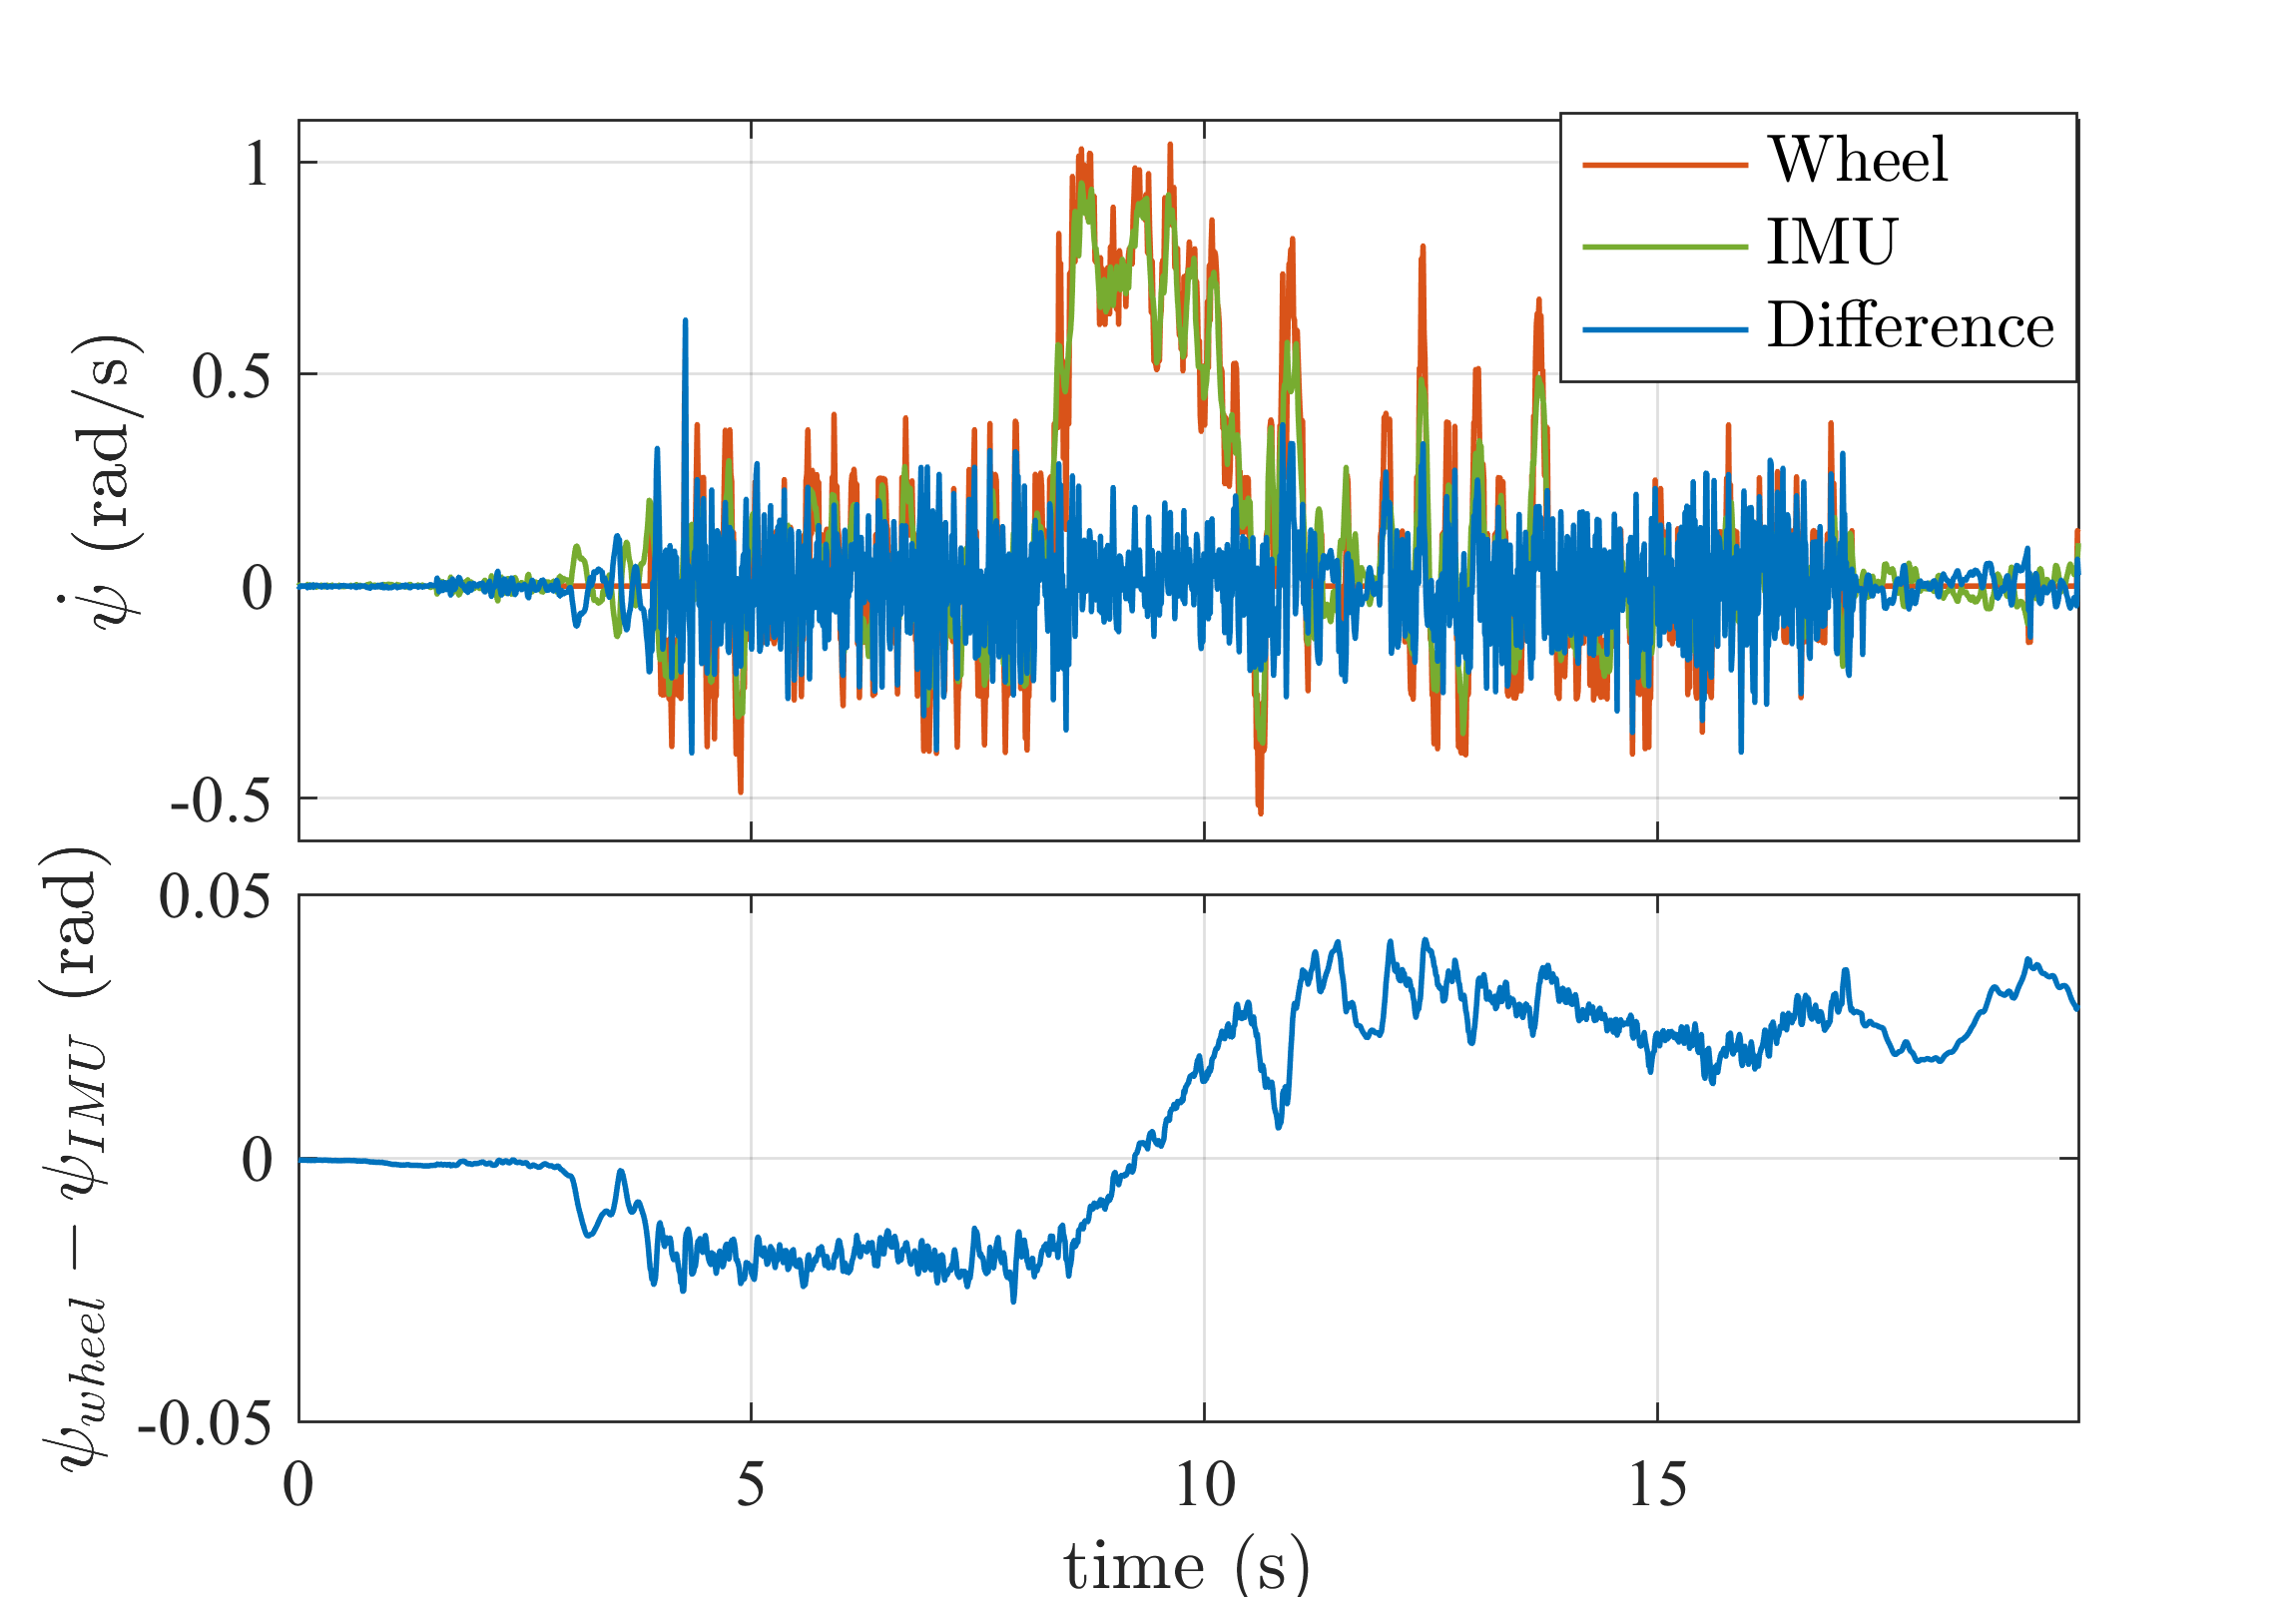
\includegraphics[width = 1.0\linewidth]{media/odometry_angle_diff.png}
    \caption{Yaw angle and angular velocity from wheel odometry and gyro.}
    \label{fig:odometry_angle_diff}
\end{figure}

\begin{figure}[hbt!]
    \centering
    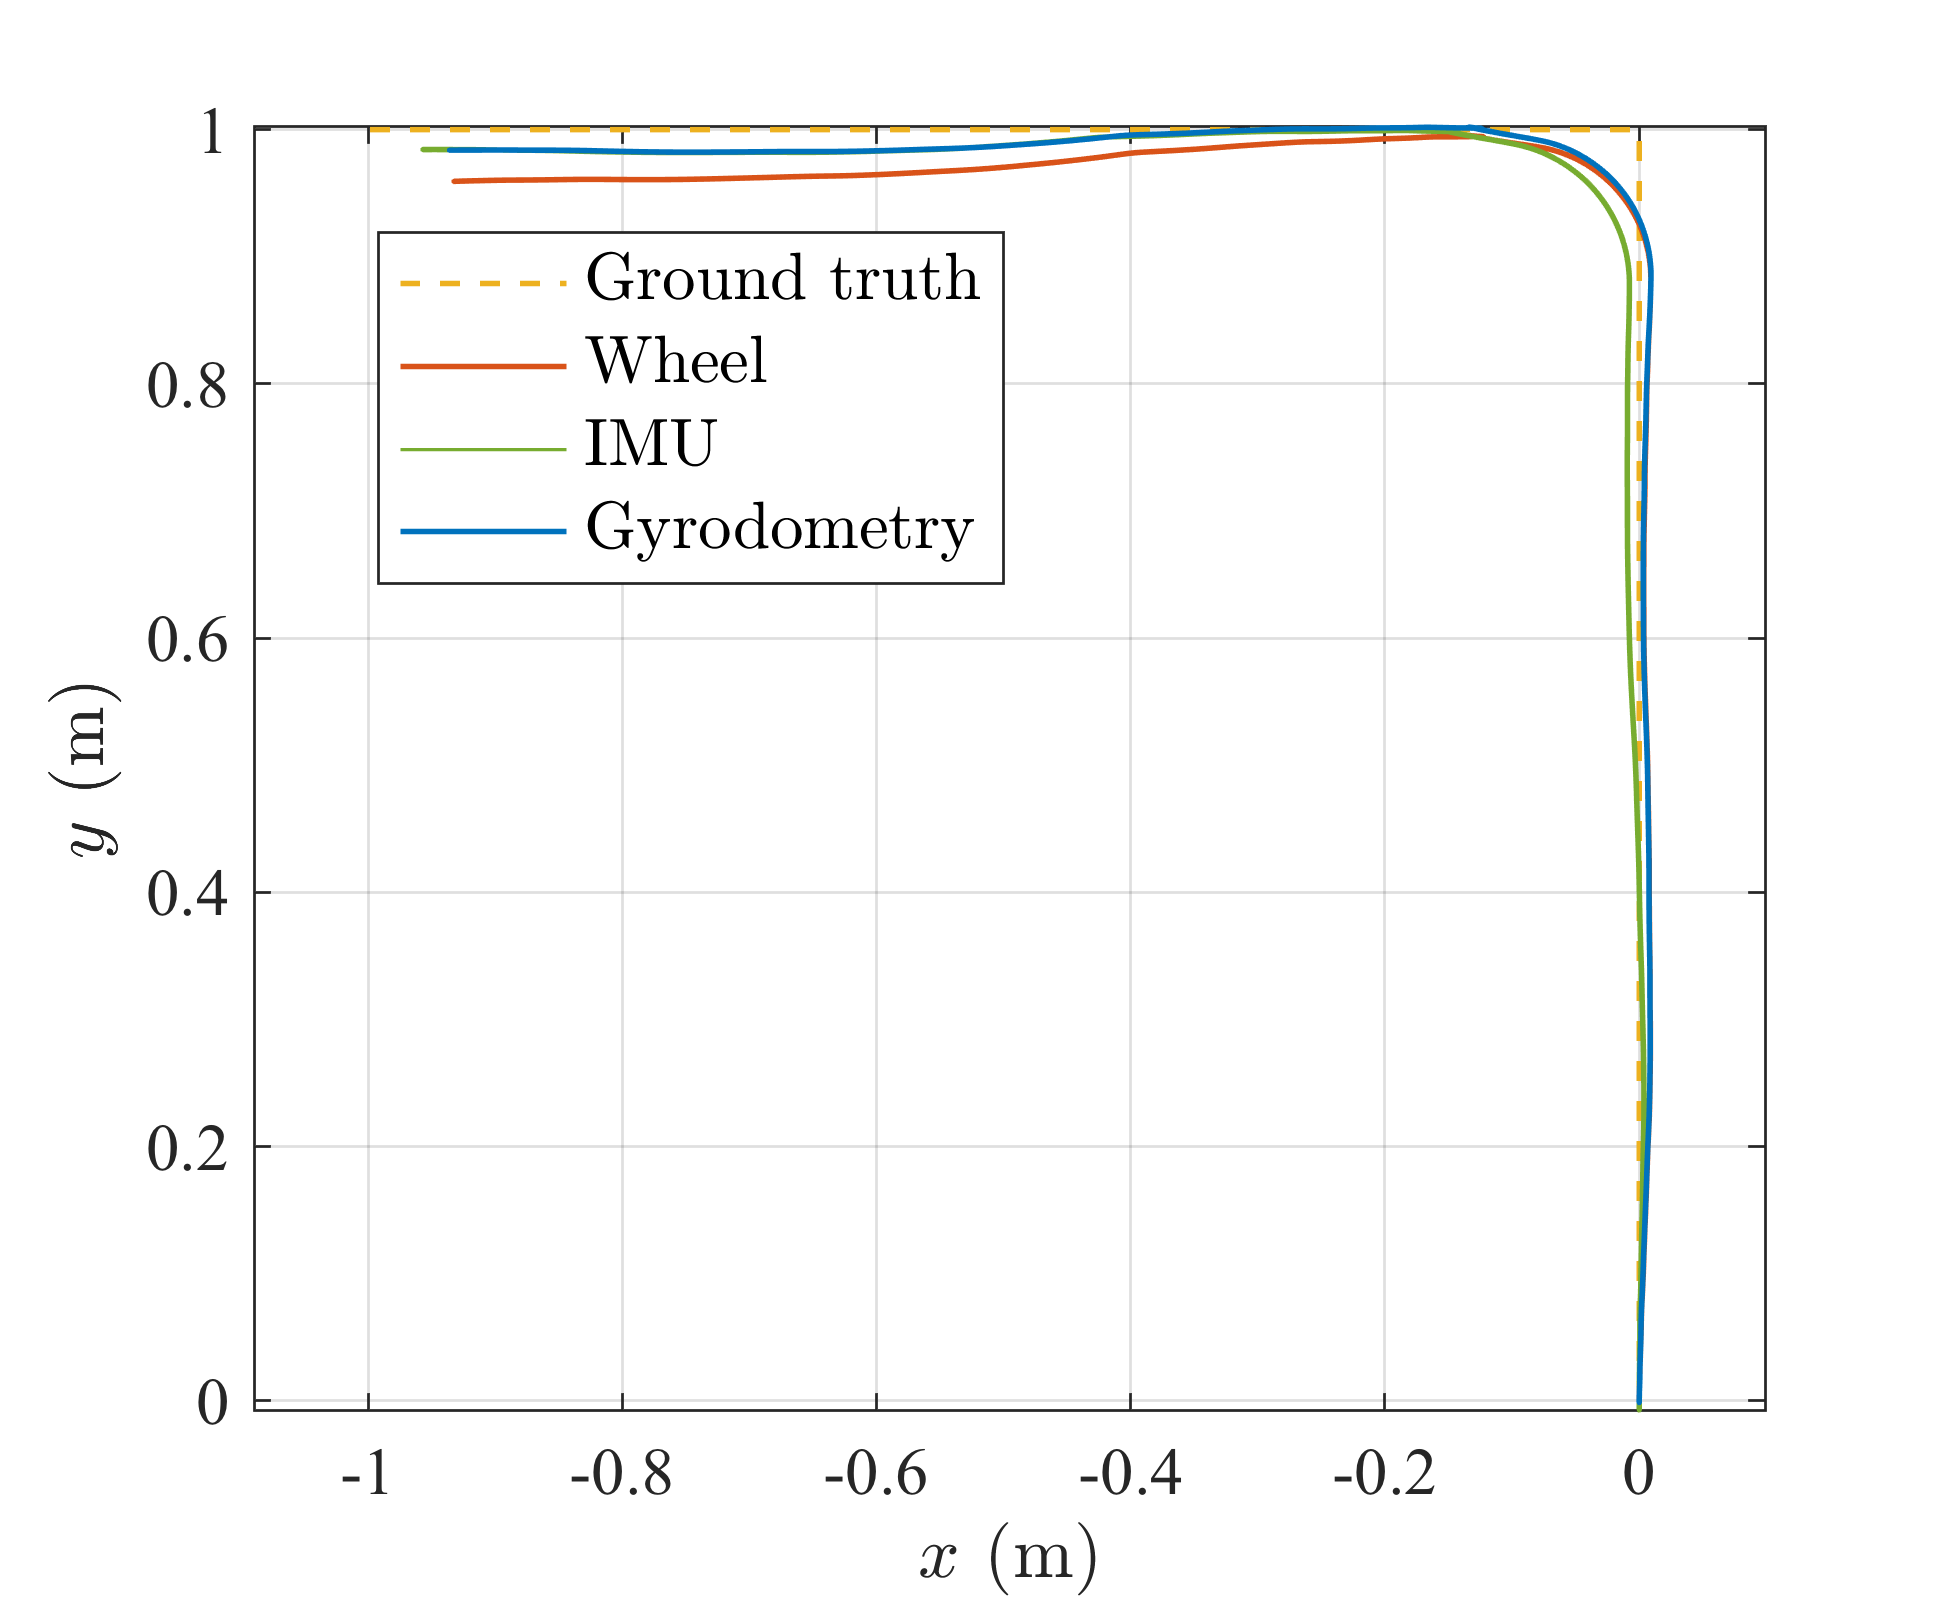
\includegraphics[width = 0.9\linewidth]{media/odometry_traj.png}
    \caption{Odometry results in different modes. The ground truth might be inaccurate during the turning process.}
    \label{fig:odometry_traj}
\end{figure}

\begin{figure}[hbt!]
    \centering
    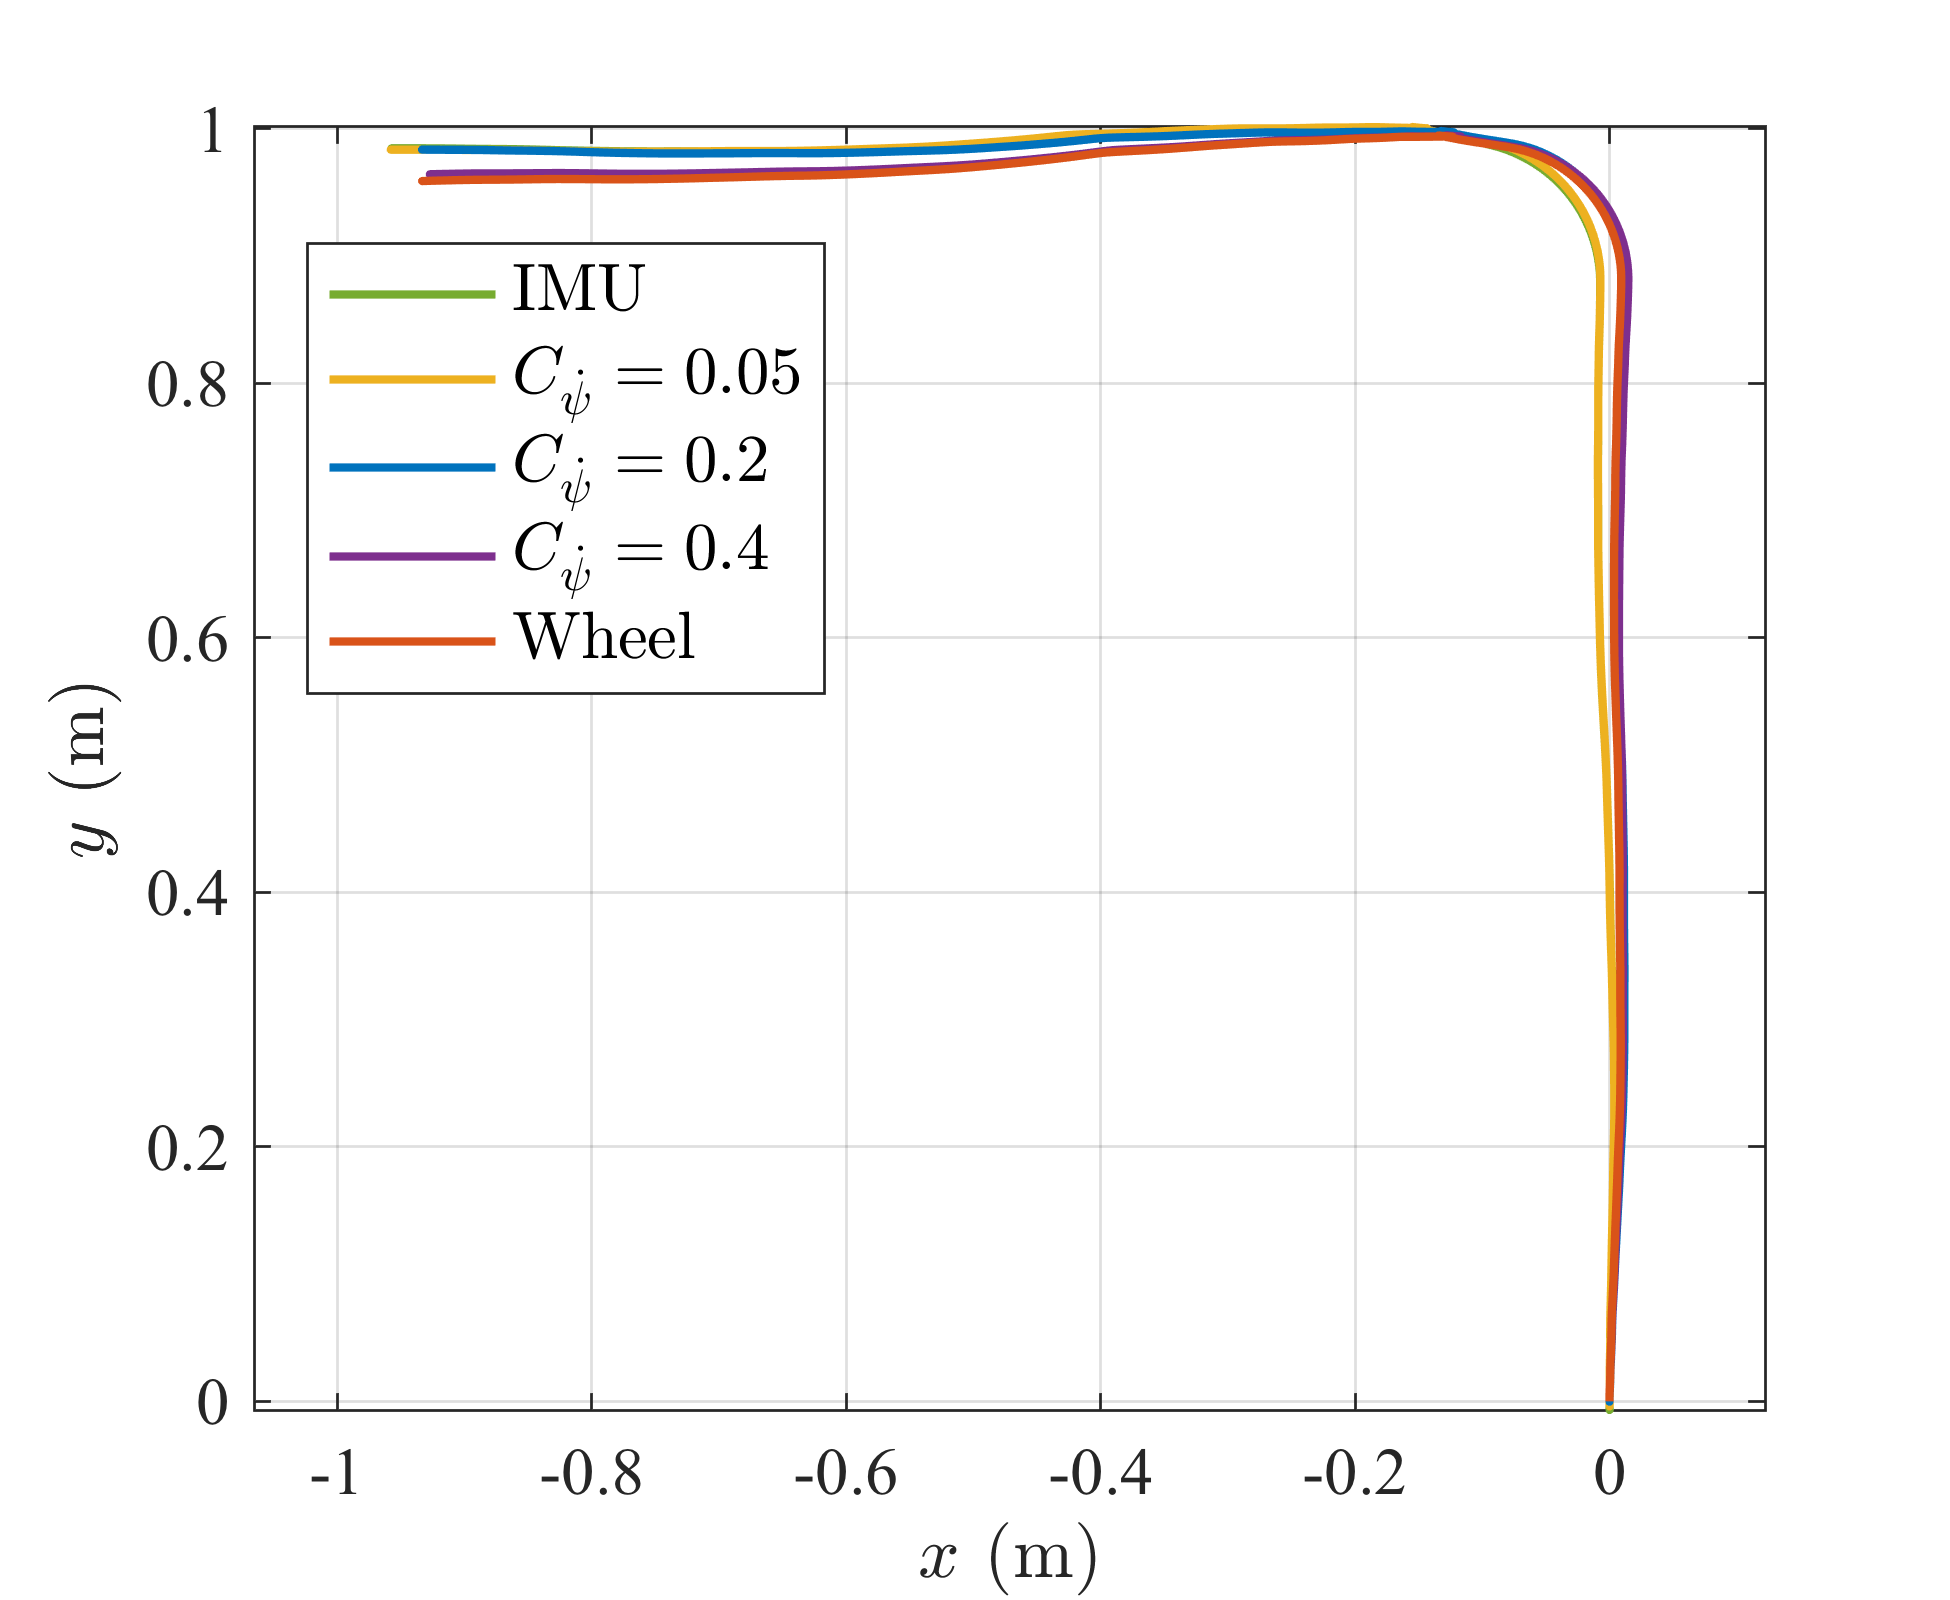
\includegraphics[width = 1.0\linewidth]{media/odometry_tune.png}
    \caption{Gyrodometry results with different \(C_{\dot{\psi}}\) (unit: rad/s) computed in MATLAB. The line of ``IMU" overlaps with ``\(C_{\dot{\psi}}\) = 0.05".}
    \label{fig:odometry_tune}
\end{figure}